% Created by tikzDevice version 0.12.6 on 2026-08-03 04:28:39
% !TEX encoding = UTF-8 Unicode
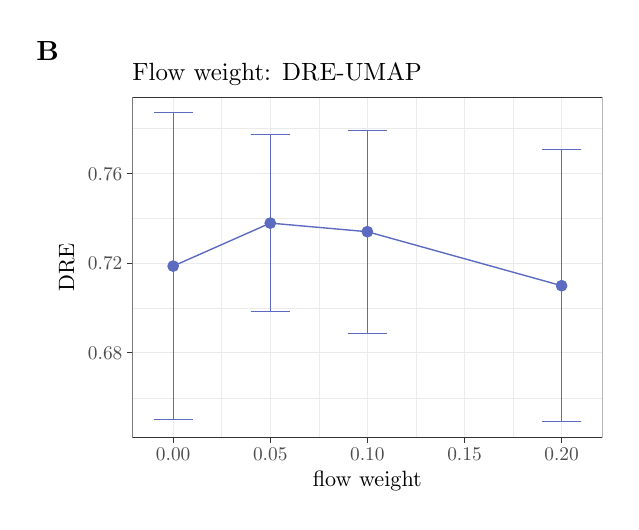
\begin{tikzpicture}[x=1pt,y=1pt]
\definecolor{fillColor}{RGB}{255,255,255}
\path[use as bounding box,fill=fillColor,fill opacity=0.00] (0,0) rectangle (210.78,171.36);
\begin{scope}
\path[clip] (  1.11,  1.87) rectangle (209.67,169.49);
\definecolor{drawColor}{RGB}{255,255,255}
\definecolor{fillColor}{RGB}{255,255,255}

\path[draw=drawColor,line width= 0.4pt,line join=round,line cap=round,fill=fillColor] (  1.11,  1.87) rectangle (209.67,169.49);
\end{scope}
\begin{scope}
\path[clip] ( 37.84, 23.34) rectangle (207.67,146.20);
\definecolor{fillColor}{RGB}{255,255,255}

\path[fill=fillColor] ( 37.84, 23.34) rectangle (207.67,146.20);
\definecolor{drawColor}{gray}{0.92}

\path[draw=drawColor,line width= 0.2pt,line join=round] ( 37.84, 37.62) --
	(207.67, 37.62);

\path[draw=drawColor,line width= 0.2pt,line join=round] ( 37.84, 70.05) --
	(207.67, 70.05);

\path[draw=drawColor,line width= 0.2pt,line join=round] ( 37.84,102.47) --
	(207.67,102.47);

\path[draw=drawColor,line width= 0.2pt,line join=round] ( 37.84,134.90) --
	(207.67,134.90);

\path[draw=drawColor,line width= 0.2pt,line join=round] ( 70.12, 23.34) --
	( 70.12,146.20);

\path[draw=drawColor,line width= 0.2pt,line join=round] (105.21, 23.34) --
	(105.21,146.20);

\path[draw=drawColor,line width= 0.2pt,line join=round] (140.30, 23.34) --
	(140.30,146.20);

\path[draw=drawColor,line width= 0.2pt,line join=round] (175.39, 23.34) --
	(175.39,146.20);

\path[draw=drawColor,line width= 0.4pt,line join=round] ( 37.84, 53.83) --
	(207.67, 53.83);

\path[draw=drawColor,line width= 0.4pt,line join=round] ( 37.84, 86.26) --
	(207.67, 86.26);

\path[draw=drawColor,line width= 0.4pt,line join=round] ( 37.84,118.68) --
	(207.67,118.68);

\path[draw=drawColor,line width= 0.4pt,line join=round] ( 52.57, 23.34) --
	( 52.57,146.20);

\path[draw=drawColor,line width= 0.4pt,line join=round] ( 87.66, 23.34) --
	( 87.66,146.20);

\path[draw=drawColor,line width= 0.4pt,line join=round] (122.75, 23.34) --
	(122.75,146.20);

\path[draw=drawColor,line width= 0.4pt,line join=round] (157.84, 23.34) --
	(157.84,146.20);

\path[draw=drawColor,line width= 0.4pt,line join=round] (192.93, 23.34) --
	(192.93,146.20);
\definecolor{drawColor}{RGB}{92,107,192}

\path[draw=drawColor,line width= 0.5pt,line join=round] ( 52.57, 85.20) --
	( 87.66,100.74) --
	(122.75, 97.63) --
	(192.93, 78.12);
\definecolor{fillColor}{RGB}{92,107,192}

\path[draw=drawColor,line width= 0.3pt,line join=round,line cap=round,fill=fillColor] ( 52.57, 85.20) circle (  1.97);

\path[draw=drawColor,line width= 0.3pt,line join=round,line cap=round,fill=fillColor] ( 87.66,100.74) circle (  1.97);

\path[draw=drawColor,line width= 0.3pt,line join=round,line cap=round,fill=fillColor] (122.75, 97.63) circle (  1.97);

\path[draw=drawColor,line width= 0.3pt,line join=round,line cap=round,fill=fillColor] (192.93, 78.12) circle (  1.97);

\path[draw=drawColor,line width= 0.3pt,line join=round] ( 45.56,140.61) --
	( 59.59,140.61);

\path[draw=drawColor,line width= 0.3pt,line join=round] ( 52.57,140.61) --
	( 52.57, 29.79);

\path[draw=drawColor,line width= 0.3pt,line join=round] ( 45.56, 29.79) --
	( 59.59, 29.79);

\path[draw=drawColor,line width= 0.3pt,line join=round] ( 80.65,132.66) --
	( 94.68,132.66);

\path[draw=drawColor,line width= 0.3pt,line join=round] ( 87.66,132.66) --
	( 87.66, 68.82);

\path[draw=drawColor,line width= 0.3pt,line join=round] ( 80.65, 68.82) --
	( 94.68, 68.82);

\path[draw=drawColor,line width= 0.3pt,line join=round] (115.73,134.40) --
	(129.77,134.40);

\path[draw=drawColor,line width= 0.3pt,line join=round] (122.75,134.40) --
	(122.75, 60.85);

\path[draw=drawColor,line width= 0.3pt,line join=round] (115.73, 60.85) --
	(129.77, 60.85);

\path[draw=drawColor,line width= 0.3pt,line join=round] (185.91,127.33) --
	(199.95,127.33);

\path[draw=drawColor,line width= 0.3pt,line join=round] (192.93,127.33) --
	(192.93, 28.92);

\path[draw=drawColor,line width= 0.3pt,line join=round] (185.91, 28.92) --
	(199.95, 28.92);
\definecolor{drawColor}{gray}{0.20}

\path[draw=drawColor,line width= 0.4pt,line join=round,line cap=round] ( 37.84, 23.34) rectangle (207.67,146.20);
\end{scope}
\begin{scope}
\path[clip] (  0.00,  0.00) rectangle (210.78,171.36);
\definecolor{drawColor}{gray}{0.30}

\node[text=drawColor,anchor=base east,inner sep=0pt, outer sep=0pt, scale=  0.70] at ( 34.24, 51.42) {0.68};

\node[text=drawColor,anchor=base east,inner sep=0pt, outer sep=0pt, scale=  0.70] at ( 34.24, 83.85) {0.72};

\node[text=drawColor,anchor=base east,inner sep=0pt, outer sep=0pt, scale=  0.70] at ( 34.24,116.27) {0.76};
\end{scope}
\begin{scope}
\path[clip] (  0.00,  0.00) rectangle (210.78,171.36);
\definecolor{drawColor}{gray}{0.20}

\path[draw=drawColor,line width= 0.4pt,line join=round] ( 35.84, 53.83) --
	( 37.84, 53.83);

\path[draw=drawColor,line width= 0.4pt,line join=round] ( 35.84, 86.26) --
	( 37.84, 86.26);

\path[draw=drawColor,line width= 0.4pt,line join=round] ( 35.84,118.68) --
	( 37.84,118.68);
\end{scope}
\begin{scope}
\path[clip] (  0.00,  0.00) rectangle (210.78,171.36);
\definecolor{drawColor}{gray}{0.20}

\path[draw=drawColor,line width= 0.4pt,line join=round] ( 52.57, 21.34) --
	( 52.57, 23.34);

\path[draw=drawColor,line width= 0.4pt,line join=round] ( 87.66, 21.34) --
	( 87.66, 23.34);

\path[draw=drawColor,line width= 0.4pt,line join=round] (122.75, 21.34) --
	(122.75, 23.34);

\path[draw=drawColor,line width= 0.4pt,line join=round] (157.84, 21.34) --
	(157.84, 23.34);

\path[draw=drawColor,line width= 0.4pt,line join=round] (192.93, 21.34) --
	(192.93, 23.34);
\end{scope}
\begin{scope}
\path[clip] (  0.00,  0.00) rectangle (210.78,171.36);
\definecolor{drawColor}{gray}{0.30}

\node[text=drawColor,anchor=base,inner sep=0pt, outer sep=0pt, scale=  0.70] at ( 52.57, 14.92) {0.00};

\node[text=drawColor,anchor=base,inner sep=0pt, outer sep=0pt, scale=  0.70] at ( 87.66, 14.92) {0.05};

\node[text=drawColor,anchor=base,inner sep=0pt, outer sep=0pt, scale=  0.70] at (122.75, 14.92) {0.10};

\node[text=drawColor,anchor=base,inner sep=0pt, outer sep=0pt, scale=  0.70] at (157.84, 14.92) {0.15};

\node[text=drawColor,anchor=base,inner sep=0pt, outer sep=0pt, scale=  0.70] at (192.93, 14.92) {0.20};
\end{scope}
\begin{scope}
\path[clip] (  0.00,  0.00) rectangle (210.78,171.36);
\definecolor{drawColor}{RGB}{0,0,0}

\node[text=drawColor,anchor=base,inner sep=0pt, outer sep=0pt, scale=  0.80] at (122.75,  5.64) {flow weight};
\end{scope}
\begin{scope}
\path[clip] (  0.00,  0.00) rectangle (210.78,171.36);
\definecolor{drawColor}{RGB}{0,0,0}

\node[text=drawColor,rotate= 90.00,anchor=base,inner sep=0pt, outer sep=0pt, scale=  0.80] at ( 16.80, 84.77) {DRE};
\end{scope}
\begin{scope}
\path[clip] (  0.00,  0.00) rectangle (210.78,171.36);
\definecolor{drawColor}{RGB}{0,0,0}

\node[text=drawColor,anchor=base west,inner sep=0pt, outer sep=0pt, scale=  0.90] at ( 37.84,152.18) {Flow weight: DRE-UMAP};
\end{scope}
\begin{scope}
\path[clip] (  0.00,  0.00) rectangle (210.78,171.36);
\definecolor{drawColor}{RGB}{0,0,0}

\node[text=drawColor,anchor=base,inner sep=0pt, outer sep=0pt, scale=  1.00] at (  7.20,159.49) {\bfseries B};
\end{scope}
\end{tikzpicture}
